\documentclass[fleqn]{article}
\oddsidemargin 0.0in
\textwidth 6.0in
\thispagestyle{empty}
\usepackage{import}
\usepackage{amsmath}
\usepackage{graphicx}
\usepackage{flexisym}
\usepackage{calligra}
\usepackage{amssymb}
\usepackage{bigints} 
\usepackage[english]{babel}
\usepackage[utf8x]{inputenc}
\usepackage{float}
\usepackage[colorinlistoftodos]{todonotes}


\DeclareMathAlphabet{\mathcalligra}{T1}{calligra}{m}{n}
\DeclareFontShape{T1}{calligra}{m}{n}{<->s*[2.2]callig15}{}
\newcommand{\scriptr}{\mathcalligra{r}\,}
\newcommand{\boldscriptr}{\pmb{\mathcalligra{r}}\,}

\definecolor{hwColor}{HTML}{1a0252}

\begin{document}

  \begin{titlepage}

    \newcommand{\HRule}{\rule{\linewidth}{0.5mm}}

    \center


    \textsc{\LARGE Arizona State University}\\[1.5cm]

    \textsc{\LARGE Quantum Physics II}\\[1.5cm]


    \begin{figure}
      
\includegraphics[width=\linewidth]{asu.png}
    \end{figure}


    \HRule \\[0.4cm]
    { \huge \bfseries Problem Set 1}\\[0.4cm] 
    \HRule \\[1.5cm]

    \textbf{Behnam Amiri}

    \bigbreak

    \textbf{Prof: Onur Erten}

    \bigbreak


    \textbf{{\large \today}\\[2cm]}

    \vfill

  \end{titlepage}

  \begin{enumerate}
    \item \textbf{(2-8)} The ether-wind theory of the Michelson-Morely experiment is discussed in the text for 
    the special case where the arms of the inter-ferometer are parallel and perpendicular to the wind. Consider
    the general case for an angular setting $\theta$ as shown (see the figure). Prove that, for equal arms of length
    $l$, the time difference for the two paths is given to a good approximation by
    $$\delta t(\theta)=\dfrac{v^2 l}{c^3} cos(2 \theta)$$
    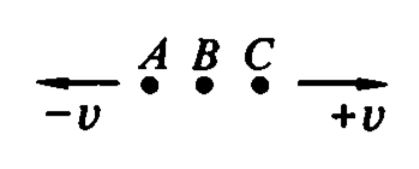
\includegraphics[height=4cm, width=4cm]{1.JPG}

      \textcolor{hwColor}{
        The Michelson–Morley experiment was an attempt to detect the existence of the luminiferous aether, 
        a supposed medium permeating space that was thought to be the carrier of light waves.
        \\
        As we will see at the end of this experiment, the exact length of the two arms are have direct 
        effect on the interference of the waves that get to the telescope. Since the setting up the exact length 
        for the two arms can get very hard (physically) and the lengths have some difference that can manifest 
        itself in the interference pattern. To get around this issue, we can rotate the entire setup by some degree $\theta$.
        \\
        \\
        \textbf{Note:} Page 54 of the textbook mentions that the light traveling from glass plate P to any of the mirrors
        and back must be aimed into the wind at such an angle that \textbf{the resultant velocity is along the path of P and the mirror}.
      }

      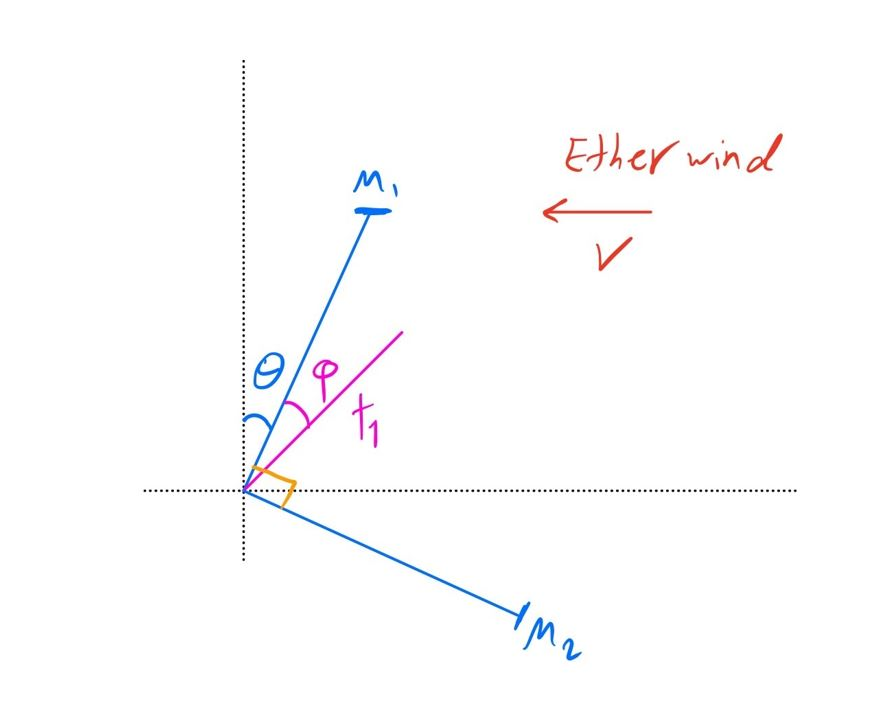
\includegraphics[height=6cm, width=8cm]{2.JPG}

      \textcolor{hwColor}{
        $
          sin(\phi)=sin(\dfrac{\pi}{2}-\theta)=cos(\theta)
          \\
          \\
        $
        Let's start off with the speed of light from the origin to $M_1$ and $M_2$.
        \\
        \\
        $
          \begin{cases}
            sin(\phi)=\dfrac{v}{c} cos(\theta) ~~~~~ \textbf{For} ~~ M_1
            \\
            \\
            sin(\phi)=\dfrac{v}{c} sin(\theta) ~~~~~ \textbf{For} ~~ M_2
          \end{cases}
          \\
          \\
          \\
          \therefore ~~~~
          \begin{cases}
            V_1=c cos(\phi)=c \sqrt{1-sin^2(\phi)}=c \sqrt{1-\left(\dfrac{v}{c} cos(\theta)\right)^2}
            \\
            \\
            V_2=c cos(\phi)=c \sqrt{1-sin^2(\phi)}=c \sqrt{1-\left(\dfrac{v}{c} sin(\theta)\right)^2}
          \end{cases}
        $
        \\
        \\
        \\
        Now by having the velocity of light for each path, we can calculate the time:
        \\
        \\
        $
          \begin{cases}
            t_1=\dfrac{2l}{V_1}=\dfrac{2l}{c \sqrt{1-\left(\dfrac{v}{c} cos(\theta)\right)^2}}
            \\
            \\
            t_2=\dfrac{2l}{V_2}=\dfrac{2l}{c \sqrt{1-\left(\dfrac{v}{c} sin(\theta)\right)^2}}
          \end{cases}
          \\
          \\
          \\
          \Delta t=t_2-t_1=\dfrac{2l}{c \sqrt{1-\left(\dfrac{v}{c} sin(\theta)\right)^2}}
          -\dfrac{2l}{c \sqrt{1-\left(\dfrac{v}{c} cos(\theta)\right)^2}}
          \\
          \\
          \\
          =\dfrac{2l}{c} \left[\dfrac{1}{\sqrt{1-\left(\dfrac{v}{c} sin(\theta)\right)^2}}
          -\dfrac{1}{\sqrt{1-\left(\dfrac{v}{c} cos(\theta)\right)^2}}\right]
          \\
          \\
          \\
          =\dfrac{2l}{c} \left[
            \left(1-\left(\dfrac{v}{c}\right)^2 sin^2(\theta)\right)^{-1/2}
            -\left(1-\left(\dfrac{v}{c}\right)^2 cos^2(\theta)\right)^{-1/2}
          \right]
          \\
          \\
          \\
          \approxeq \dfrac{2l}{c} \left[
            \left(1-\dfrac{1}{2} \left(\dfrac{v}{c}\right)^2 sin^2(\theta)\right)
            -\left(1+\dfrac{1}{2} \left(\dfrac{v}{c}\right)^2 cos^2(\theta) \right)
          \right]
          \\
          \\
          \\
          =\dfrac{2l}{c} \left[\dfrac{1}{2} \left(\dfrac{v}{c}\right)^2 \left(-sin(\theta)+cos^2(\theta)\right)\right]
          \\
          \\
          \\
          \therefore ~~~~ \Delta t \approxeq \dfrac{lv^2}{c^3} cos(2 \theta) ~~~ \checkmark
        $ 
      }

    \item \textbf{(3-4)} Given that 
    $$x^'=\gamma (x-vt)$$
    and 
    $$t^'=\gamma (t-\dfrac{vx}{c^2})$$
    derive the equations for $x$ and $t$ in terms of $x^'$ and $t^'$.

      % \textcolor{hwColor}{

      % }

    \item \textbf{(4-4)} Our galaxy is about $10^5$ light-years across, and the most energetic particles known
    have an energy of about $10^{19} ~ eV$. How long would it take a proton with this energy to traverse the galaxy
    as measured in the rest frame of 
    \begin{enumerate}
      \item The galaxy?

        % \textcolor{hwColor}{

        % }

      \item The particle?

        % \textcolor{hwColor}{

        % }

    \end{enumerate}

  \end{enumerate}

\end{document}